\chapter{テスト文章}\label{sec:first}

Lorem ipsum \cite{LoremipsWikipedia:online} (ロレム・イプサム,略してリプサム lipsum ともいう)とは,出版,ウェブデザイン,グラフィックデザインなどの諸分野において使用されている典型的なダミーテキストである.

\begin{quote}
  Lorem ipsum dolor sit amet, consectetur adipiscing elit, sed do eiusmod tempor incididunt ut labore et dolore magna aliqua. Ut enim ad minim veniam, quis nostrud exercitation ullamco laboris nisi ut aliquip ex ea commodo consequat. Duis aute irure dolor in reprehenderit in voluptate velit esse cillum dolore eu fugiat nulla pariatur.
\end{quote}

デカルト座標で,点 \((a, b)\) を中心とする半径 \(r\) の円は,次式の陰関数で与えられる.

\[
(x - a)^2 + (y - b)^2 = r^2
\label{eq:circle}
\]

図\ref{fig:image} は,Unsplash \footnotemark から引用している.

\footnotetext{\url{https://unsplash.com/}}

\begin{figure}[tb]
\centering
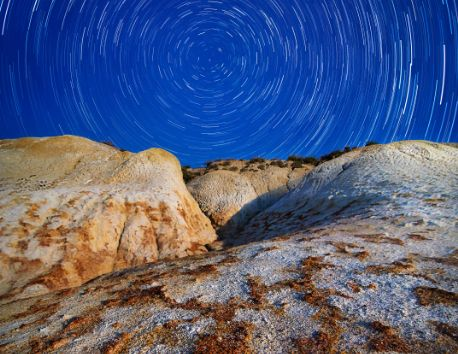
\includegraphics[
  keepaspectratio=true,
  width=0.85\linewidth,
  height=0.15\paperheight
]{../assets/sample.jpg}
\caption{サンプル}
\label{fig:image}
\end{figure}
